%&<latex>
\documentclass[letterpaper,12pt]{article}
\pdfoutput=1

%%%%%%%%%%%%%%%%%%%%%%%%%%%%%%%%%%%%%%%%%%%%%%%%%%%%%%%%%%%%
%% preamble %%%%%%%%%%%%%%%%%%%%%%%%%%%%%%%%%%%%%%%%%%%%%%%%
\pdfpagewidth = 8.5in
\pdfpageheight = 11.0in
\usepackage[left=1in,right=1in,top=1in,bottom=1in]{geometry}

\pagestyle{plain}
\pagenumbering{arabic}
\usepackage[nodisplayskipstretch]{setspace}
\usepackage[fleqn]{amsmath}
\usepackage{amssymb}
\usepackage{graphicx}
\usepackage[hyphens]{url}
\usepackage{verbatim}
\usepackage[title]{appendix}
\usepackage{indentfirst}
\usepackage{booktabs}
\usepackage{multirow}
\usepackage{ragged2e}
\usepackage{upgreek}
\usepackage[T1]{fontenc}
\usepackage[titles]{tocloft}
\usepackage{xspace}
% xcolor allows rowcolors for tables
\usepackage[table,x11names,dvipsnames,table]{xcolor}
% \usepackage[usenames]{color}
\usepackage{ifthen}
\usepackage{cancel}
\usepackage{array}
\usepackage{tabulary}
\usepackage{authblk}
\usepackage{tikz}
\usepackage{pdflscape}
\usepackage[normalem]{ulem}

%% Set up color palettes %%%%%%%%%%%%%%%%%%%%%%%%%%%%%%%%%%%%%%%%%%%%
% Color palette GreenOrange_6 from
% https://jiffyclub.github.io/palettable/tableau/
\definecolor{pgreen}     {RGB}{50,162,81}
\definecolor{porange}    {RGB}{255,127,15}
\definecolor{pblue}      {RGB}{60,183,204}
\definecolor{pyellow}    {RGB}{255,217,74}
\definecolor{pteal}      {RGB}{57,115,124}
\definecolor{pauburn}    {RGB}{184,90,13}
%%%%%%%%%%%%%%%%%%%%%%%%%%%%%%%%%%%%%%%%%%%%%%%%%%%%%%%%%%%%%%%%%%%%%
\definecolor{mygray}{gray}{0.9}

\usepackage{hyperref}
\hypersetup{pdfborder={0 0 0},
            colorlinks=true,
            % colorlinks=false,
            urlcolor=porange,
            linkcolor=pauburn,
            citecolor=pteal}

\usepackage[capitalize]{cleveref}
\newcommand{\crefrangeconjunction}{--}

% Set up line numbering; using lineno to number lines of paragraphs with
% equations sanely
\usepackage[right, mathlines]{lineno}
\setlength\linenumbersep{1cm}
\def\linenumberfont{\normalfont\scriptsize\sffamily}

% Set up caption formatting
\usepackage{subcaption}
\usepackage[format=plain, labelsep=period, singlelinecheck=false, skip=4pt, font=sf, font=footnotesize]{caption}
\DeclareCaptionLabelFormat{noSpace}{{#1}{#2}}
\DeclareCaptionListFormat{figList}{Figure {#2}.}
\DeclareCaptionListFormat{sFigList}{Figure S{#2}.}

\newenvironment{mytitle}
 {\parskip=0pt\par\nopagebreak\centering\LARGE\slshape}
 {\par\noindent\ignorespacesafterend}

% Define tightly formated list environments via enumitem
\usepackage{enumitem}
\newenvironment{tightItemize}{%
\begin{itemize}[noitemsep, topsep=0pt, parsep=0pt, partopsep=0pt]}
{\end{itemize}}

\newenvironment{veryTightItemize}{%
\begin{itemize}[noitemsep, topsep=0pt, parsep=0pt, partopsep=0pt, leftmargin=*]}
{\end{itemize}}

\newenvironment{tightEnumerate}{%
\begin{enumerate}[noitemsep, topsep=0pt, parsep=0pt, partopsep=0pt]}
{\end{enumerate}}

\newenvironment{veryTightEnumerate}{%
\begin{enumerate}[noitemsep, topsep=0pt, parsep=0pt, partopsep=0pt, leftmargin=*]}
{\end{enumerate}}

% Redefine abstract environment as a list to control left/right margins
% From https://tex.stackexchange.com/a/151589
\renewenvironment{abstract}
 {\small
  \begin{center}
  \bfseries \abstractname\vspace{-.5em}\vspace{0pt}
  \end{center}
  \list{}{%
    \setlength{\leftmargin}{5mm}%
    \setlength{\rightmargin}{\leftmargin}%
  }%
  \item\relax}
 {\endlist}

\newcommand{\jroedit}[2]{\sout{#1}{\color{red}{#2}}}
% \newcommand{\jroedit}[2]{#2}
\newcommand{\jrocomment}[1]{({\color{pgreen}{JRO's comment:}} \textbf{\color{pgreen}{#1}})}

\newcommand{\citationNeeded}{\textcolor{magenta}{\textbf{[CITATION NEEDED]}}\xspace}
\newcommand{\tableNeeded}{\textcolor{magenta}{\textbf{[TABLE NEEDED]}}\xspace}
\newcommand{\figureNeeded}{\textcolor{magenta}{\textbf{[FIGURE NEEDED]}}\xspace}
\newcommand{\highLight}[1]{\textcolor{magenta}{\MakeUppercase{#1}}}

\newcommand{\fig}{Figure\xspace}
\newcommand{\figs}{Figures\xspace}
\newcommand{\tbl}{Table\xspace}
\newcommand{\tbls}{Tables\xspace}

\newcommand{\datasets}{data sets\xspace}
\newcommand{\dataset}{data set\xspace}

\newcommand{\ignore}[1]{}
\newcommand{\addTail}[1]{\textit{#1}.---}
\newcommand{\super}[1]{\ensuremath{^{\textrm{#1}}}}
\newcommand{\sub}[1]{\ensuremath{_{\textrm{#1}}}}
\newcommand{\dC}{\ensuremath{^\circ{\textrm{C}}}}
\newcommand{\tn}{\tabularnewline}
\newcommand{\spp}[1]{\textit{#1}}

\providecommand{\e}[1]{\ensuremath{\times 10^{#1}}}

\newcommand{\change}[2]{{\color{red} #2}\xspace}
\newcommand{\thought}[1]{\textcolor{purple}{THOUGHT: #1}}

\newcommand{\widthFigure}[5]{\begin{figure}[htbp]
\begin{center}
    \includegraphics[width=#1\textwidth]{#2}
    \captionsetup{#3}
    \caption{#4}
    \label{#5}
    \end{center}
    \end{figure}}

\newcommand{\heightFigure}[5]{\begin{figure}[htbp]
\begin{center}
    \includegraphics[height=#1\textheight]{#2}
    \captionsetup{#3}
    \caption{#4}
    \label{#5}
    \end{center}
    \end{figure}}

\newcommand{\smartFigure}[5]{%
    \begin{figure}[htbp]
        \begin{center}
            \includegraphics[width=\textwidth,height=#1\textheight,keepaspectratio]{#2}
            \captionsetup{#3}
            \caption{#4}
            \label{#5}
        \end{center}
    \end{figure}
}

\newcommand{\mFigure}[4]{\smartFigure{#1}{#2}{listformat=figList}{#3}{#4}\clearpage}
\newcommand{\embedHeightFigure}[4]{\heightFigure{#1}{#2}{listformat=figList}{#3}{#4}}
\newcommand{\embedWidthFigure}[4]{\widthFigure{#1}{#2}{listformat=figList}{#3}{#4}}
\newcommand{\siFigure}[4]{\smartFigure{#1}{#2}{name=Figure S, labelformat=noSpace, listformat=sFigList}{#3}{#4}\clearpage}

%% macro to make long strings breakable over lines
\makeatletter
\def\breakable#1{\xHyphen@te#1$\unskip}
\def\xHyphen@te{\@ifnextchar${\@gobble}{\sw@p{\allowbreak{}\xHyphen@te}}}
% \def\xHyphen@te{\@ifnextchar${\@gobble}{\sw@p{\hskip 0pt plus 1pt\xHyphen@te}}}
\def\sw@p#1#2{#2#1}
\makeatother

\newcommand{\accuracyscatterplotannotations}[1]{For each plot, the
    root-mean-square error (RMSE) and the proportion of estimates for which the
    95\% credible interval contained the true value---$p(#1 \in
    \textrm{CI})$---is given.
}
\newcommand{\neventsplotannotations}{For each plot,
    the proportion of simulation replicates for which the number of events with
    the largest posterior probability matched the true number of
    events---$p(\hat{\nevents} = \nevents)$---is shown in the upper left
    corner,
    the median posterior probability of the correct number of events across all
    simulations---$\widetilde{p(\nevents|\alldata)}$---is shown in the upper
    right corner, and
    the proportion of simulations for which the true divergence model was
    included in the 95\% credible set---$p(\nevents \in
    \textrm{CS})$---is shown in the lower right.
}
\newcommand{\neventsbarplotannotations}{For each plot, the following summary
    statistics are shown:
    the proportion of simulation replicates for which the number of events with
    the largest posterior probability matched the true number of
    events---$p(\hat{\nevents} = \nevents)$---,
    the median posterior probability of the correct number of events across all
    simulations---$\widetilde{p(\nevents|\alldata)}$---, and
    the proportion of simulations for which the true divergence model was
    included in the 95\% credible set---$p(\nevents \in
    \textrm{CS})$---.
}
\newcommand{\neventsshadingdescription}{The number of simulation replicates
    that fall within each possible cell of true versus estimated numbers of
    events is shown, and cells with more replicates are shaded darker.
}

\newcommand{\given}{\ensuremath{\,|\,}\xspace}
\newcommand{\pr}{\ensuremath{p}}

\newcommand{\data}{\ensuremath{D}\xspace}
\newcommand{\model}[1][]{\ensuremath{M_{#1}}\xspace}
\newcommand{\parameters}[1][]{\ensuremath{\Theta_{#1}}\xspace}
\newcommand{\parameter}[1][]{\ensuremath{\theta_{#1}}\xspace}
\newcommand{\diff}[1]{\ensuremath{\mathrm{d}#1}}

\newcommand{\distgamma}{\ensuremath{\textrm{Gamma}}\xspace}
\newcommand{\distexponential}{\ensuremath{\textrm{Exponential}}\xspace}
\newcommand{\distbeta}{\ensuremath{\textrm{Beta}}\xspace}
\newcommand{\dgamma}[2]{\ensuremath{\distgamma(\textrm{shape} = #1, \textrm{mean} = #2)}}
\newcommand{\dexponential}[1]{\ensuremath{\distexponential(\textrm{mean} = #1)}}
\newcommand{\dbeta}[2]{\ensuremath{\distbeta(\alpha = #1, \beta = #2)}}

\newcommand{\ncomparisons}{\ensuremath{\mathcal{N}}\xspace}
\newcommand{\nevents}[1][]{\ensuremath{K_{#1}}\xspace}
\newcommand{\nexistingcats}{\ensuremath{\mathcal{K}}\xspace}
\newcommand{\nloci}[1][]{\ensuremath{m_{#1}}\xspace}

\newcommand{\observedallelecount}[1][]{\ensuremath{n_{#1}}\xspace}
\newcommand{\observedredallelecount}[1][]{\ensuremath{r_{#1}}\xspace}

\newcommand{\nodeallelecount}[2]{\ensuremath{n_{#1}^{#2}}}
\newcommand{\noderedallelecount}[2]{\ensuremath{r_{#1}^{#2}}}

\newcommand{\allelecount}[1][]{\ensuremath{\nodeallelecount{#1}{}}\xspace}
\newcommand{\redallelecount}[1][]{\ensuremath{\noderedallelecount{#1}{}}\xspace}

\newcommand{\leafallelecounts}[1][]{\ensuremath{\mathbf{n}_{#1}}\xspace}
\newcommand{\leafredallelecounts}[1][]{\ensuremath{\mathbf{r}_{#1}}\xspace}
\newcommand{\maxleafallelecounts}{\ensuremath{\textrm{max}(\mathbf{n})}\xspace}

\newcommand{\comparisondata}[1][]{\ensuremath{D_{#1}}\xspace}
\newcommand{\alldata}[1][]{\ensuremath{\mathbf{D}}\xspace}

\newcommand{\branchindex}{\ensuremath{x}\xspace}
\newcommand{\allelecountbottom}[1][\branchindex]{\nodeallelecount{#1}{B}}
\newcommand{\allelecounttop}[1][\branchindex]{\nodeallelecount{#1}{T}}
\newcommand{\redallelecountbottom}[1][\branchindex]{\noderedallelecount{#1}{B}}
\newcommand{\redallelecounttop}[1][\branchindex]{\noderedallelecount{#1}{T}}

\newcommand{\cpp}{\upshape\texttt{C++}\xspace}
\newcommand{\ecoevolity}{\upshape\texttt{ecoevolity}\xspace}
\newcommand{\Ecoevolity}{\upshape\texttt{Ecoevolity}\xspace}
\newcommand{\dppmsbayes}{\upshape\texttt{dpp-msbayes}\xspace}
\newcommand{\simcoevolity}{\upshape\texttt{simcoevolity}\xspace}
\newcommand{\sumcoevolity}{\upshape\texttt{sumcoevolity}\xspace}
\newcommand{\pycoevolity}{\upshape\texttt{pycoevolity}\xspace}
\newcommand{\dpprobs}{\upshape\texttt{DPprobs}\xspace}

\newcommand{\wunif}{WU\xspace}

\newcommand{\rgmurate}{\ensuremath{u}\xspace}
\newcommand{\grmurate}{\ensuremath{v}\xspace}
\newcommand{\murate}[1][]{\ensuremath{\mu_{#1}}\xspace}
\newcommand{\murates}[1][]{\ensuremath{\boldsymbol{\mu}_{#1}}\xspace}
\newcommand{\gfreq}[1][]{\ensuremath{\pi_{#1}}\xspace}
\newcommand{\gfreqs}[1][]{\ensuremath{\boldsymbol{\pi}_{#1}}\xspace}

\newcommand{\comparisonetime}[1][]{\ensuremath{t_{#1}}\xspace}
\newcommand{\comparisonetimes}[1][]{\ensuremath{\mathbf{t}_{#1}}\xspace}
\newcommand{\etime}[1][]{\ensuremath{\tau_{#1}}\xspace}
\newcommand{\etimes}[1][]{\ensuremath{\boldsymbol{\tau}_{#1}}\xspace}
\newcommand{\etimemodel}[1][]{\ensuremath{T_{#1}}\xspace}
\newcommand{\etimesets}{\ensuremath{\mathcal{T}}\xspace}
\newcommand{\genetree}[1][]{\ensuremath{g_{#1}}\xspace}
\newcommand{\sptree}[1][]{\ensuremath{S_{#1}}\xspace}
\newcommand{\sptrees}[1][]{\ensuremath{\mathbf{S}_{#1}}\xspace}

\newcommand{\descendantpopindex}[1]{\ensuremath{D{#1}}}
\newcommand{\rootpopindex}[1][]{\ensuremath{R{#1}}\xspace}
\newcommand{\epopsize}[1][]{\ensuremath{N_{e}^{#1}}\xspace}
\newcommand{\sepopsize}[1][]{\ensuremath{N}\xspace}
\newcommand{\comparisonpopsizes}[1][]{\ensuremath{\mathbb{N}_{e}{#1}}\xspace}
\newcommand{\collectionpopsizes}[1][]{\ensuremath{\mathbf{N_{e}}_{#1}}\xspace}
\newcommand{\rootrelativepopsize}{\ensuremath{R_{\epopsize[\rootpopindex]}}\xspace}

\newcommand{\dirp}{\ensuremath{\textrm{DP}}\xspace}
\newcommand{\concentration}{\ensuremath{\alpha}\xspace}
\newcommand{\discount}{\ensuremath{d}\xspace}
\newcommand{\splitweight}{\ensuremath{s}\xspace}
\newcommand{\basedistribution}{\ensuremath{H}\xspace}
\newcommand{\gshape}{\ensuremath{k}\xspace}
\newcommand{\gscale}{\ensuremath{\theta}\xspace}

\newcommand{\proposed}{\ensuremath{^{\prime}}\xspace}
\newcommand{\tuningparameter}{\ensuremath{\lambda}\xspace}
\newcommand{\uniformdeviate}{\ensuremath{u}\xspace}


\newcommand{\ifdoublespacing}[2]{#1}
% \newcommand{\ifdoublespacing}[2]{#2}
\newcommand{\iflinenumbers}[2]{#1}
% \newcommand{\iflinenumbers}[2]{#2}
% \newcommand{\ifragged}[2]{#1}
\newcommand{\ifragged}[2]{#2}

\captionsetup[figure]{listformat=figList}

\usepackage[round]{natbib}
\usepackage{amsmath}
\title{The great codivergence bake off}

\author[1]{Tanner Myers}
\author[1]{Randy Klabacka}
\author[1]{Hailey Whitaker}
\author[1]{Tashitso Anamza}
\author[1]{Claire Tracy}
\author[1]{Jamie R.\ Oaks \thanks{Corresponding author: \href{mailto:joaks@auburn.edu}{\tt joaks@auburn.edu}}}
\affil[1]{Department of Biological Sciences \& Museum of Natural History, Auburn University, Auburn, Alabama 36849}

\date{\today}

\makeatletter
\let\msTitle\@title
\let\msAuthor\@author
\let\msDate\@date
\makeatother
%%%%%%%%%%%%%%%%%%%%%%%%%%%%%%%%%%%%%%%%%%%%%%%%%%%%%%%%%%%%
%%%%%%%%%%%%%%%%%%%%%%%%%%%%%%%%%%%%%%%%%%%%%%%%%%%%%%%%%%%%

\begin{document}

\ifragged{
\raggedright
}{}

\iflinenumbers{
\begin{linenumbers}
}{}

\textbf{Running head}: \uppercase{Codiv bake off}

{\let\newpage\relax\maketitle}

\newpage

\ifdoublespacing{
\doublespacing
}{}

\begin{abstract}
    Abstract here \ldots

    \vspace{6pt}
    \noindent\textbf{KEY WORDS:}
\end{abstract}

\newpage

\section{Introduction}

\section{Methods}

\subsection{Analyses of simulated data}

\subsection{Empirical analyses}

\section{Results}

\subsection{Simulation results}

\begin{figure}[htbp]
    \begin{center}
        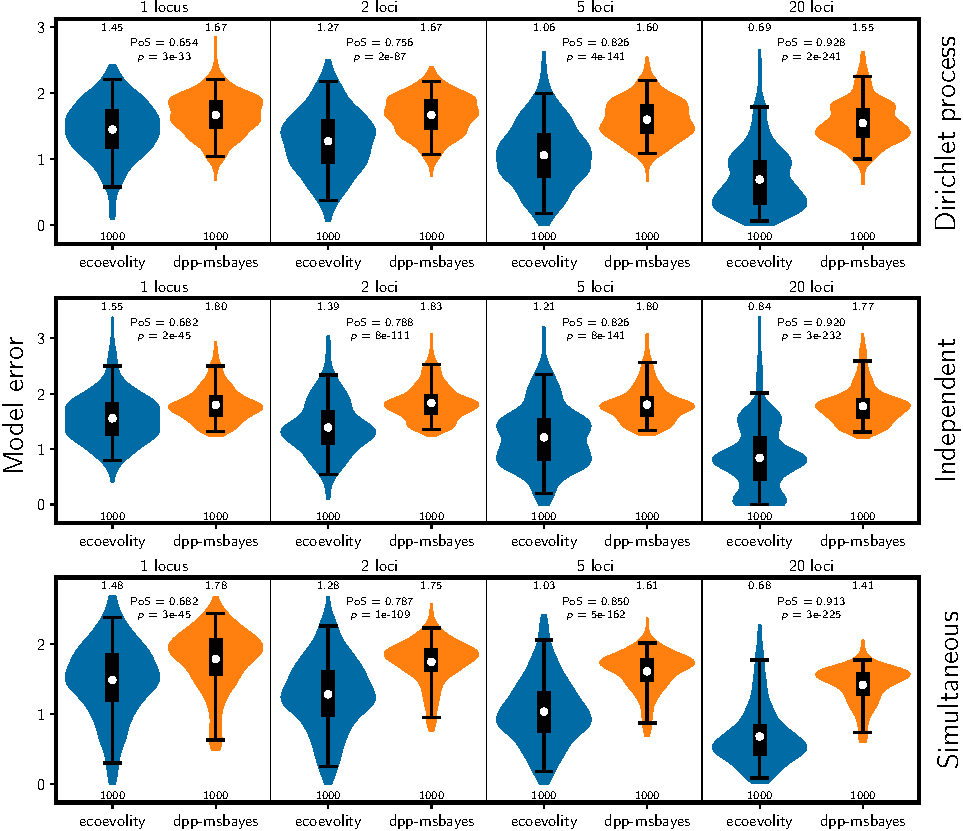
\includegraphics[width=\textwidth,height=\textheight,keepaspectratio]{../images/from-project-repo/plots/tex-plot-grids/grid-model-distance-cropped.pdf}
        \caption{
            \Ecoevolity estimates the partitioning of population pairs to
            divergence times (the divergence model) more accurately and
            precisely than \dppmsbayes across all simulated numbers of loci
            (columns) and whether the divergence model was drawn from a
            Dirichlet process (top row), or constrained so that all pairs of
            populations diverged independently (middle row) or simultaneously
            (bottom row).
            Divergence model estimation error was quantified for each
            simulation replicate using the mean partition distance
            \citep{Regnier1983,Gusfield2002} between the true divergence model
            and the posterior samples of divergence models.
            Partition distances was calculated using the Hungarian (or
            Kuhn-Munkres) algorithm
            \citep{Kuhn1955,Munkres1957}
            as implemented in \pycoevolity
            \citep[Version 0.2.11 Commit 85ea44b;][]{Oaks2018ecoevolity,PycoevolityRepoOnline},
            which relies on the Munkres Python package
            \citep[Version 1.1.4;][]{Clapper2020}.
            For each violin plot, the sample size (number of simulation
            replicates) is shown beneath and the mean is represented by the
            white dot and shown above.
            The box shows the upper and lower quartiles and the brackets
            show the 2.5th and 97.5th percentiles.
            At the top center of each plot, the results of a Mann-Whitney U
            test \citep{MannWhitney1947} are shown comparing mean model errors
            between \ecoevolity and \dppmsbayes;
            the probability of superiority \citep[PoS, the probability that
            \ecoevolity has a lower mean model error than \dppmsbayes for a
            random simulation replicate drawn from
            each;][]{WolfeHogg1971,Grissom1994} and p-value is provided.
        }
        \label{fig:modelerror}
    \end{center}
\end{figure}

\begin{figure}[htbp]
    \begin{center}
        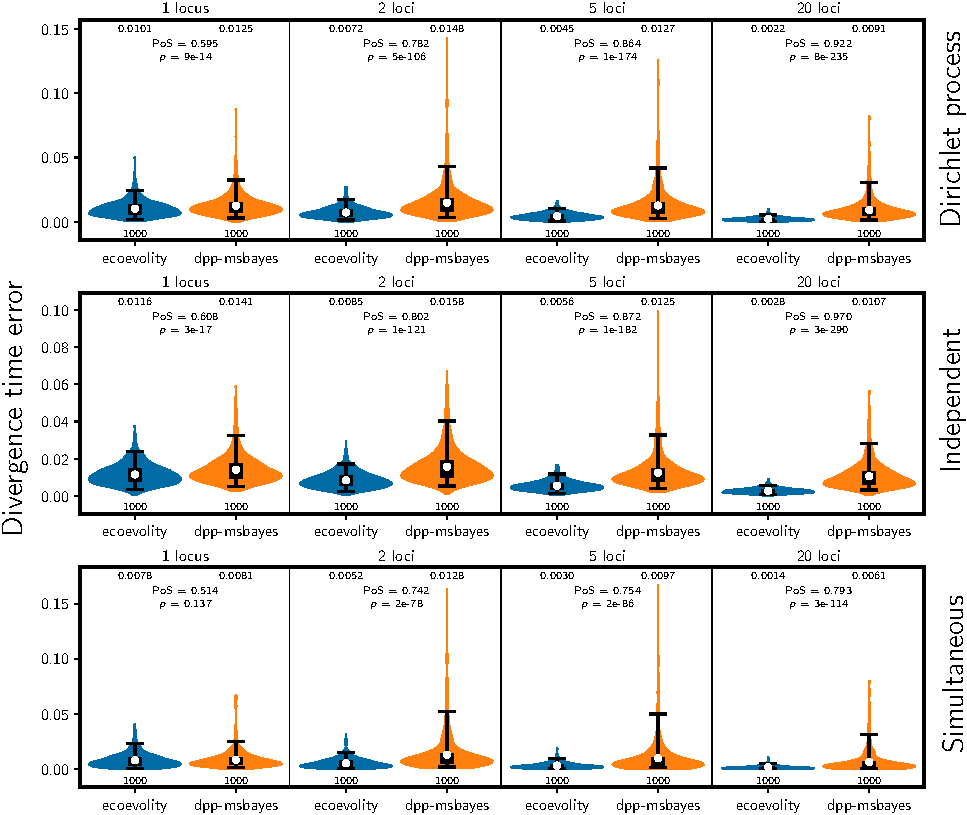
\includegraphics[width=\textwidth,height=\textheight,keepaspectratio]{../images/from-project-repo/plots/tex-plot-grids/grid-div-time-error-cropped.pdf}
        \caption{
            \Ecoevolity better estimates divergence times than \dppmsbayes
            across all simulated numbers of loci (columns) and whether the
            divergence model was drawn from a Dirichlet process (top row), or
            constrained so that all pairs of populations diverged independently
            (middle row) or simultaneously (bottom row).
            Divergence time error was quantified for each simulation replicate
            as the sum of the difference between the true and posterior mean
            divergence time across the five pairs of populations.
            For each violin plot, the sample size (number of simulation
            replicates) is shown beneath and the mean is represented by the
            white dot and shown above.
            The box shows the upper and lower quartiles and the brackets
            show the 2.5th and 97.5th percentiles.
            At the top center of each plot, the results of a Mann-Whitney U
            test \citep{MannWhitney1947} are shown comparing mean model errors
            between \ecoevolity and \dppmsbayes;
            the probability of superiority \citep[PoS, the probability that
            \ecoevolity has a lower mean model error than \dppmsbayes for a
            random simulation replicate drawn from
            each;][]{WolfeHogg1971,Grissom1994} and p-value is provided.
        }
        \label{fig:divtimeerror}
    \end{center}
\end{figure}

\begin{figure}[htbp]
    \begin{center}
        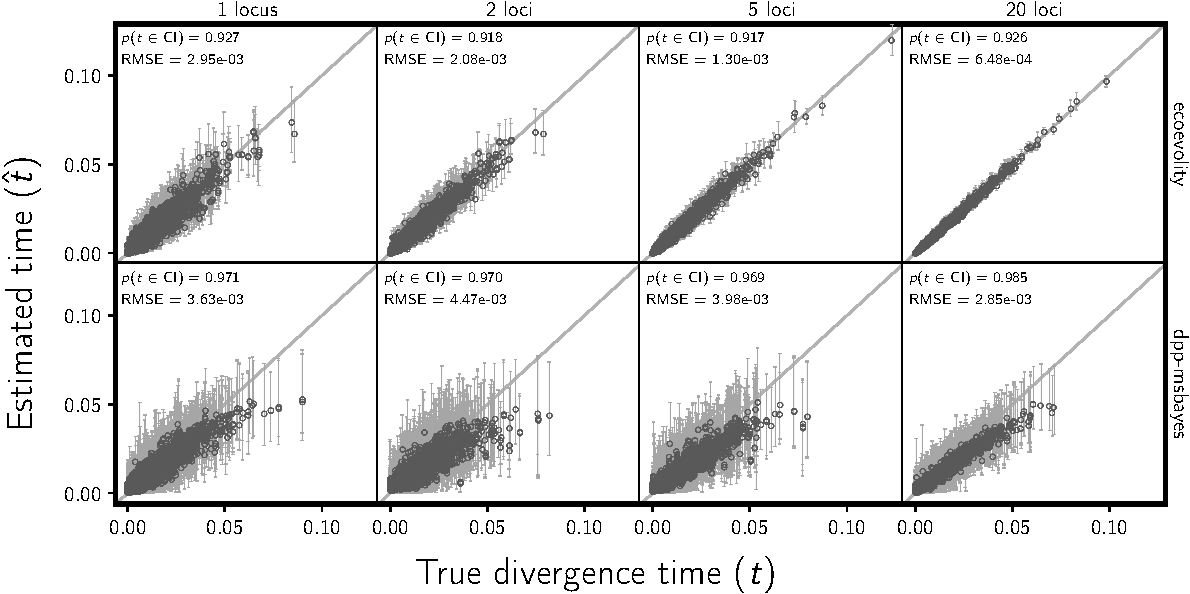
\includegraphics[width=\textwidth,height=\textheight,keepaspectratio]{../images/from-project-repo/plots/free-div-time-scatter-cropped.pdf}
        \caption{
            \Ecoevolity (top row) estimates divergence times more accurately
            and precisely than \dppmsbayes (bottom row) across all simulated
            numbers of loci (columns) for five pairs of populations simulated
            to have diverged according to a Dirichlet process.
            Each plotted circle and associated error bars represent the posterior mean
            and 95\% credible interval.
            \accuracyscatterplotannotations{\comparisonetime{}}
        }
        \label{fig:divtimeerrordp}
    \end{center}
\end{figure}

\subsection{Empirical results}


\section{Discussion}


\section{Acknowledgments}

This work was supported by funding provided to JRO from the National Science
Foundation (NSF grant number DEB 1656004).
The computational work was made possible by the Auburn University (AU) Hopper
Cluster supported by the AU Office of Information Technology and a grant of
high-performance computing resources and technical support from the Alabama
Supercomputer Authority.
This paper is contribution number \highLight{XXX} of the Auburn University
Museum of Natural History.


%TC:ignore

\bibliographystyle{evolution}
\bibliography{references}


\iflinenumbers{
\end{linenumbers}
}{}


%%%%%%%%%%%%%%%%%%%%%%%%%%%%%%%%%%%%%%%%%%%%%%%%%%%%%%%%%%%%%%%%%%
%% SUPPORTING INFO %%%%%%%%%%%%%%%%%%%%%%%%%%%%%%%%%%%%%%%%%%%%%%%
\newpage
\setcounter{figure}{0}
\setcounter{table}{0}
\setcounter{page}{1}
\setcounter{section}{0}

\captionsetup[figure]{name=Figure S, labelformat=noSpace, listformat=sFigList}
\captionsetup[table]{name=Table S, labelformat=noSpace}

\singlespacing

\section*{Supporting Information}
\hangindent=1cm
\noindent Title: \msTitle

\bigskip
{\noindent Authors: \msAuthor}

\newpage
\singlespacing

\input{si-body.tex}
\clearpage

\input{si-tables.tex}
\clearpage

\begin{figure}[htbp]
    \begin{center}
        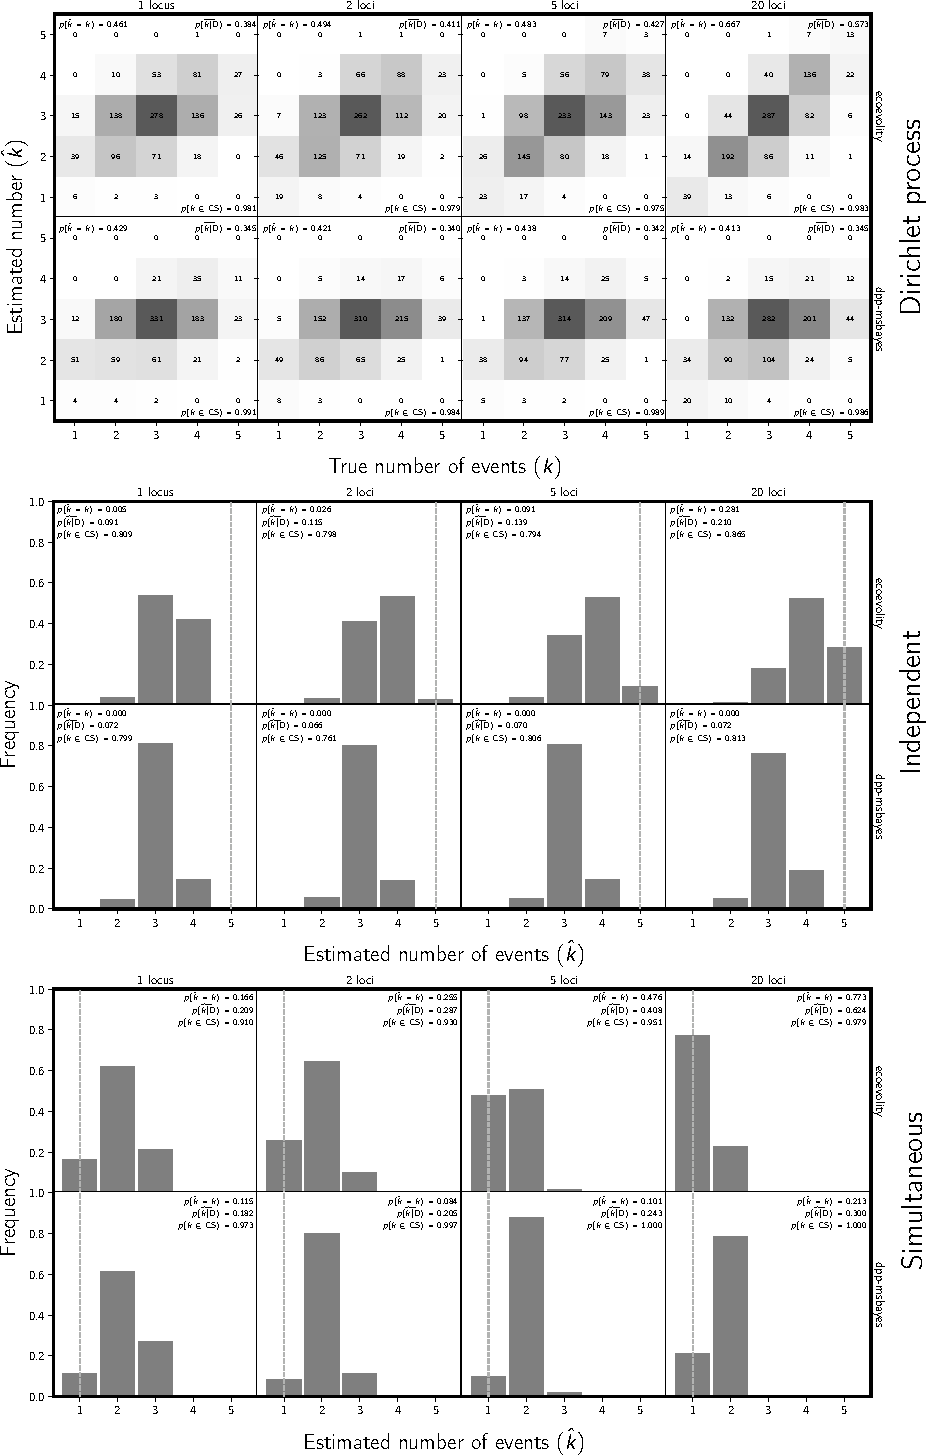
\includegraphics[width=\textwidth,height=0.9\textheight,keepaspectratio]{../images/from-project-repo/plots/tex-plot-grids/grid-nevents-cropped.pdf}
        \caption{
            \scriptsize
            \Ecoevolity better estimates the number of divergence
            events than \dppmsbayes across all simulated numbers of
            loci (columns) for five pairs of populations simulated to have
            diverged according to a Dirichlet process (top 8 plots),
            indepedently (middle 8 plots),
            or
            simultaneously (bottom 8 plots).
            \neventsshadingdescription{}
            \neventsplotannotations{}
        }
        \label{fig:nevents}
    \end{center}
\end{figure}

\clearpage

\begin{figure}[htbp]
    \begin{center}
        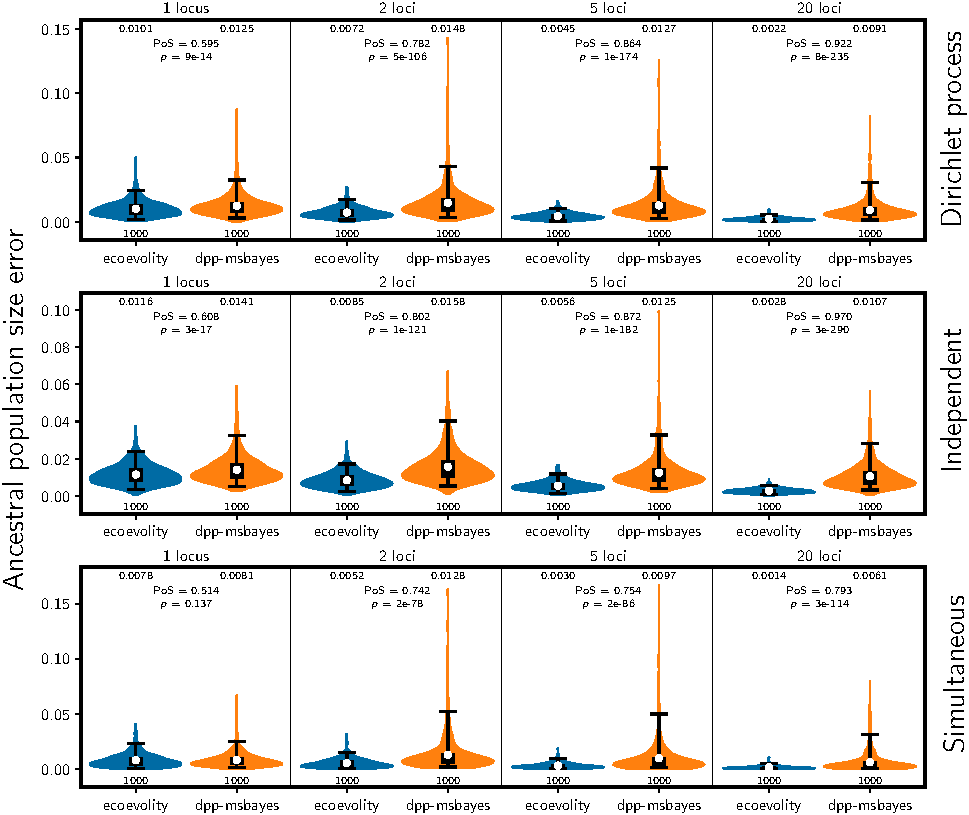
\includegraphics[width=\textwidth,height=\textheight,keepaspectratio]{../images/from-project-repo/plots/tex-plot-grids/grid-ancestral-pop-size-error-cropped.pdf}
        \caption{
            \scriptsize
            \Ecoevolity better estimates the effective size of the ancestral
            populations than \dppmsbayes across all simulated numbers of loci
            (columns) and whether the divergence model was drawn from a
            Dirichlet process (top row), or constrained so that all pairs of
            populations diverged independently (middle row) or simultaneously
            (bottom row).
            Error was quantified for each simulation replicate
            as the sum of the difference between the true and posterior mean
            population size across the five pairs of populations.
            For each violin plot, the sample size (number of simulation
            replicates) is shown beneath and the mean is represented by the
            white dot and shown above.
            The box shows the upper and lower quartiles and the brackets
            show the 2.5th and 97.5th percentiles.
            At the top center of each plot, the results of a Mann-Whitney U
            test \citep{MannWhitney1947} are shown comparing mean model errors
            between \ecoevolity and \dppmsbayes;
            the probability of superiority \citep[PoS, the probability that
            \ecoevolity has a lower mean model error than \dppmsbayes for a
            random simulation replicate drawn from
            each;][]{WolfeHogg1971,Grissom1994} and p-value is provided.
        }
        \label{fig:ancpopsizeerror}
    \end{center}
\end{figure}

\clearpage

\begin{figure}[htbp]
    \begin{center}
        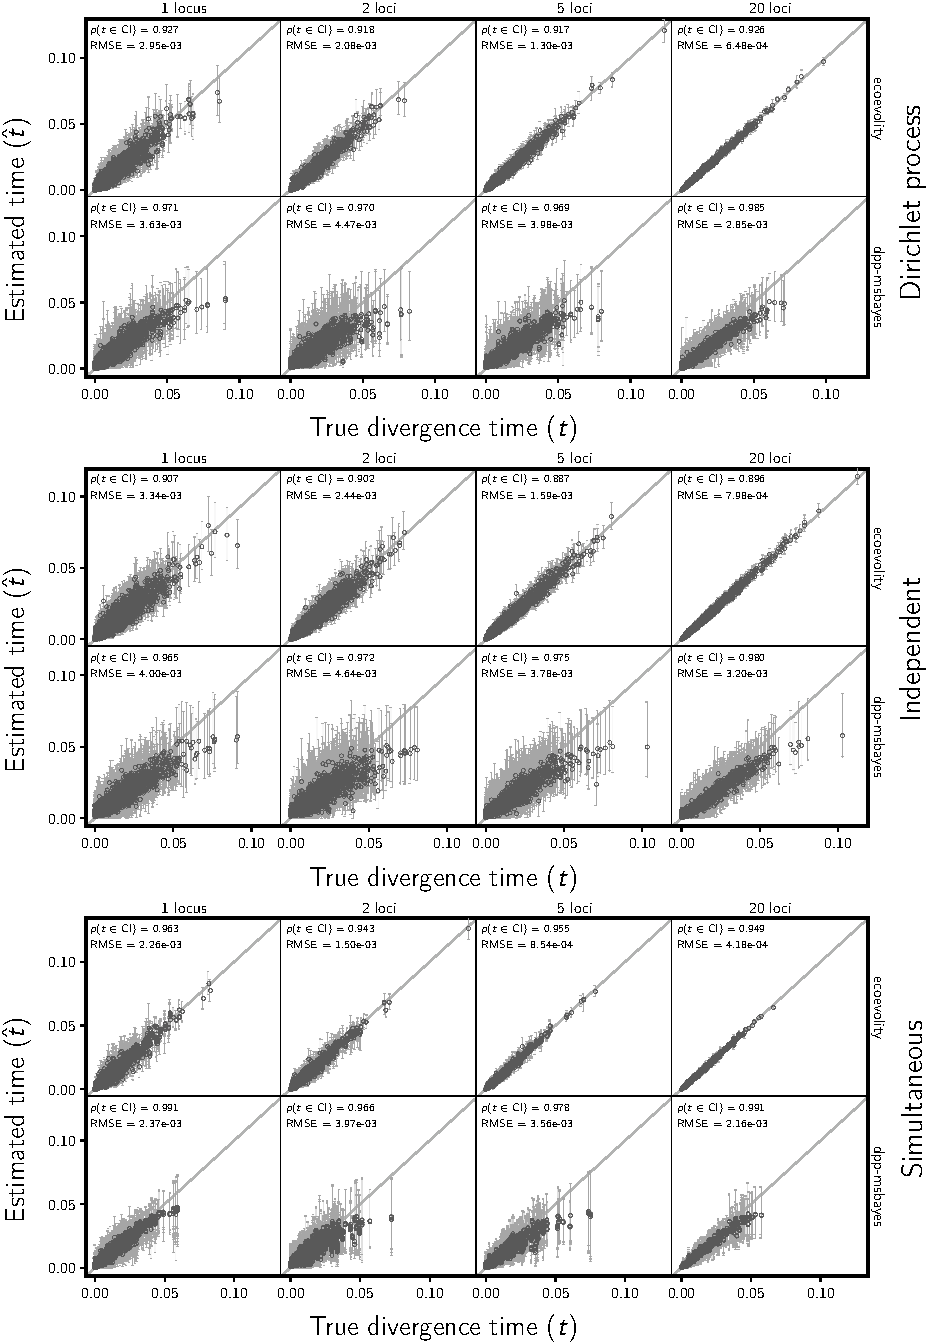
\includegraphics[width=\textwidth,height=0.9\textheight,keepaspectratio]{../images/from-project-repo/plots/tex-plot-grids/grid-div-time-scatter-cropped.pdf}
        \caption{
            \scriptsize
            \Ecoevolity estimates divergence times more accurately
            and precisely than \dppmsbayes across all simulated
            numbers of loci (columns) for five pairs of populations simulated
            to have diverged according to a dirichlet process (top 8 plots),
            independently (middle 8 plots),
            or simultaneously (bottom 8 plots).
            Each plotted circle and associated error bars represent the posterior mean
            and 95\% credible interval.
            \accuracyscatterplotannotations{\comparisonetime{}}
        }
        \label{fig:divtimescatter}
    \end{center}
\end{figure}

\clearpage

\begin{figure}[htbp]
    \begin{center}
        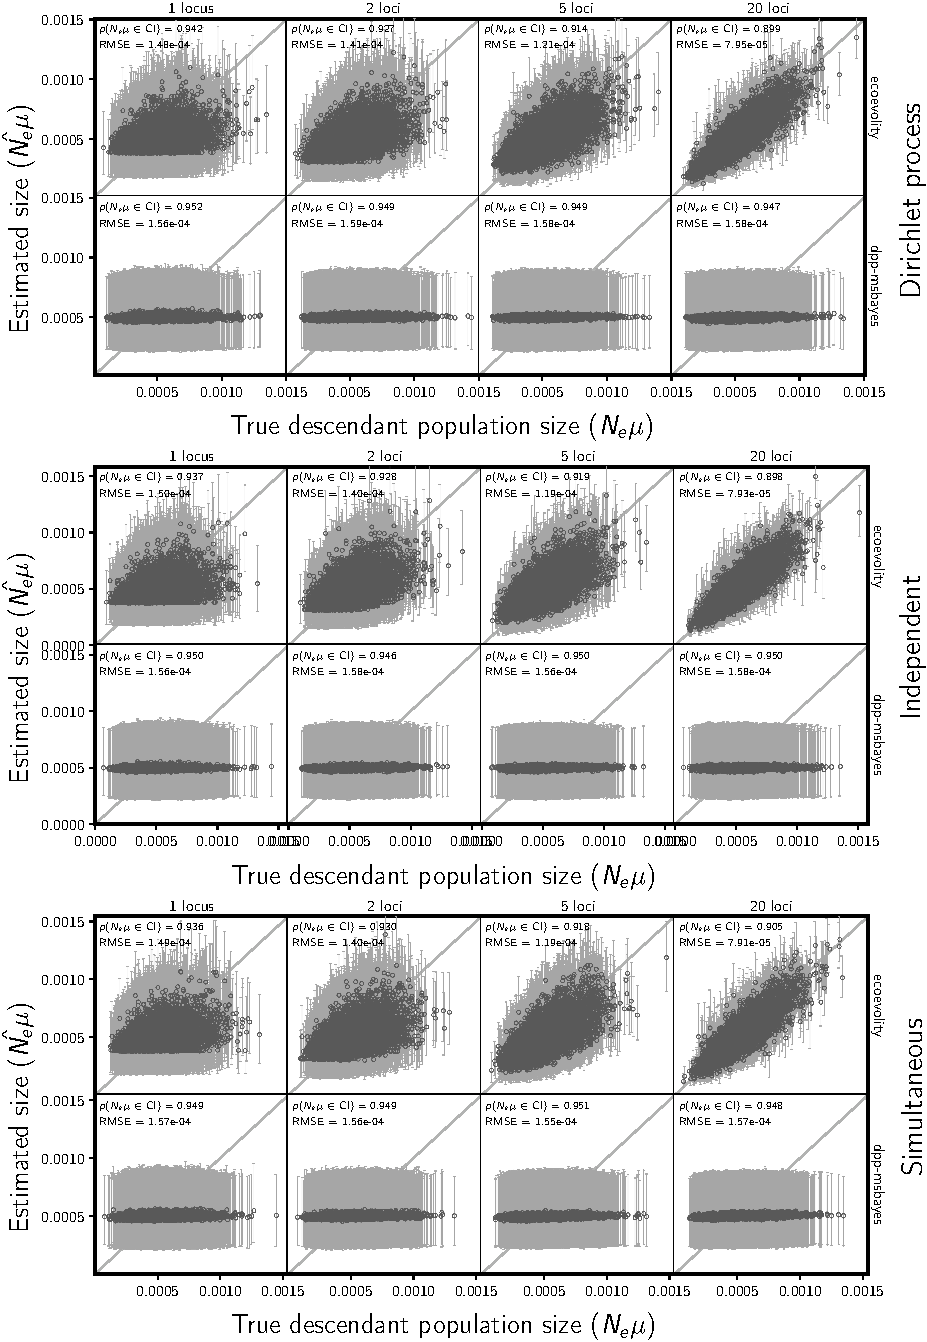
\includegraphics[width=\textwidth,height=0.9\textheight,keepaspectratio]{../images/from-project-repo/plots/tex-plot-grids/grid-leaf-pop-size-scatter-cropped.pdf}
        \caption{
            \scriptsize
            \Ecoevolity estimates the effective sizes of the
            descendant populations more accurately and precisely than
            \dppmsbayes across all simulated numbers of loci
            (columns) for five pairs of populations simulated to have diverged
            according to a Dirichlet process (top 8 plots),
            independently (middle 8 plots),
            or simultaneously (bottom 8 plots).
            Each plotted circle and associated error bars represent the posterior mean
            and 95\% credible interval.
            \accuracyscatterplotannotations{\epopsize{}}
        }
        \label{fig:leafpopsizescatter}
    \end{center}
\end{figure}

\clearpage

\begin{figure}[htbp]
    \begin{center}
        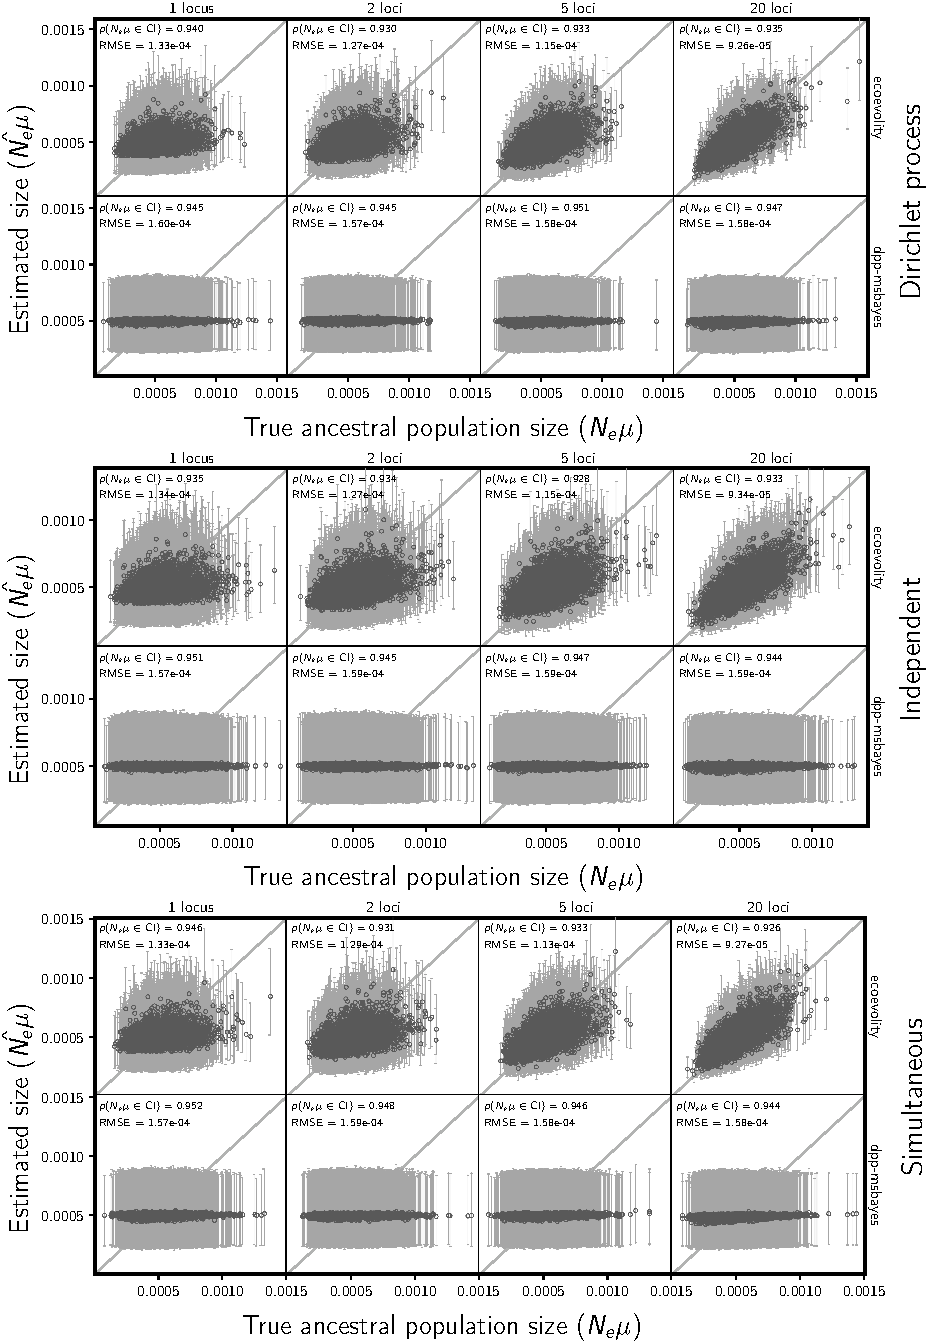
\includegraphics[width=\textwidth,height=0.9\textheight,keepaspectratio]{../images/from-project-repo/plots/tex-plot-grids/grid-root-pop-size-scatter-cropped.pdf}
        \caption{
            \Ecoevolity estimates the effective sizes of the
            ancestral populations more accurately and precisely than
            \dppmsbayes across all simulated numbers of loci
            (columns) for five pairs of populations simulated to have diverged
            according to a Dirichlet process (top 8 plots),
            independently (middle 8 plots),
            or simultaneously (bottom 8 plots).
            Each plotted circle and associated error bars represent the posterior mean
            and 95\% credible interval.
            \accuracyscatterplotannotations{\epopsize{}}
        }
        \label{fig:rootpopsizescatter}
    \end{center}
\end{figure}

\begin{figure}[htbp]
    \begin{center}
        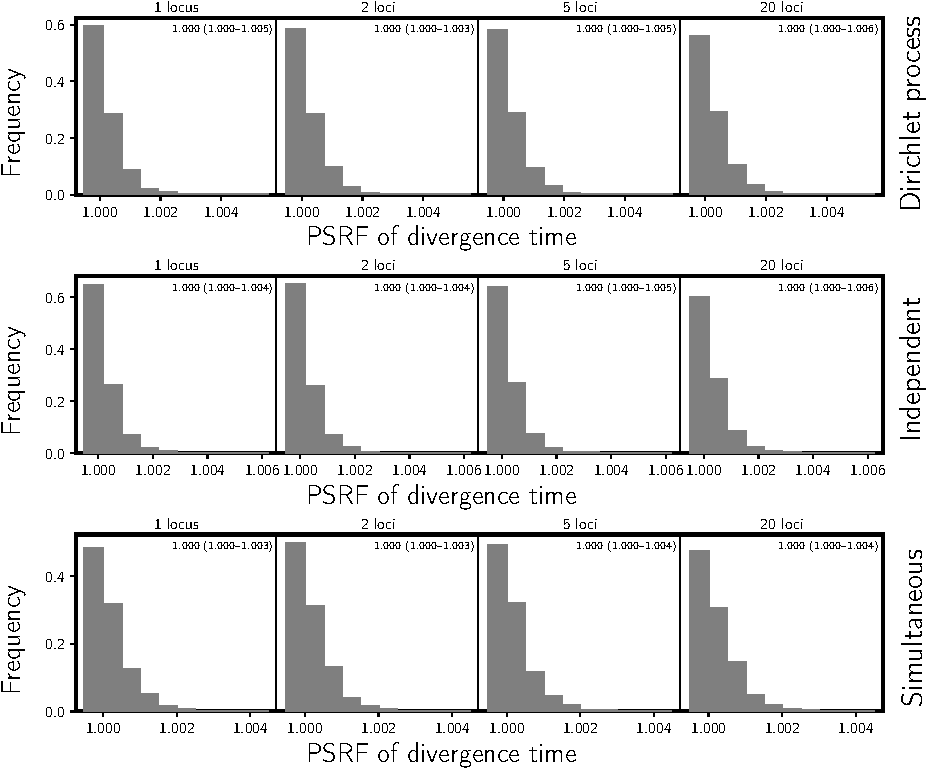
\includegraphics[width=\textwidth,height=0.9\textheight,keepaspectratio]{../images/from-project-repo/plots/tex-plot-grids/grid-psrf-div-time-histograms-cropped.pdf}
        \caption{
            The potential scale reduction factor \citep[PSRF; the square root
            of Equation 1.1 in][]{Brooks1998}
            for the divergence time parameter calculated from the last 1000
            samples of the four MCMC chains run for each simulation replicate.
            The mean PSRF across the 1000 simulation replicates is shown at the
            top right of each plot, followed by the range in parentheses.
        }
        \label{fig:psrfdivtime}
    \end{center}
\end{figure}

\begin{figure}[htbp]
    \begin{center}
        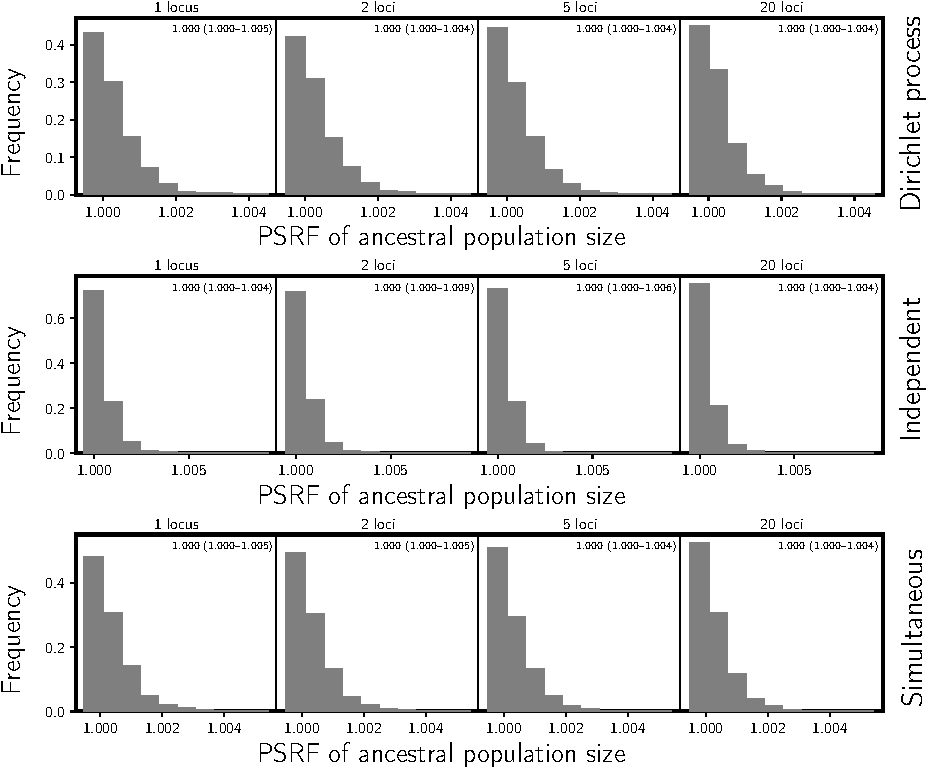
\includegraphics[width=\textwidth,height=0.9\textheight,keepaspectratio]{../images/from-project-repo/plots/tex-plot-grids/grid-psrf-root-pop-size-histograms-cropped.pdf}
        \caption{
            The potential scale reduction factor \citep[PSRF; the square root
            of Equation 1.1 in][]{Brooks1998}
            for the ancestral population size calculated from the last 1000
            samples of the four MCMC chains run for each simulation replicate.
            The mean PSRF across the 1000 simulation replicates is shown at the
            top right of each plot, followed by the range in parentheses.
        }
        \label{fig:psrfrootpopsize}
    \end{center}
\end{figure}

\begin{figure}[htbp]
    \begin{center}
        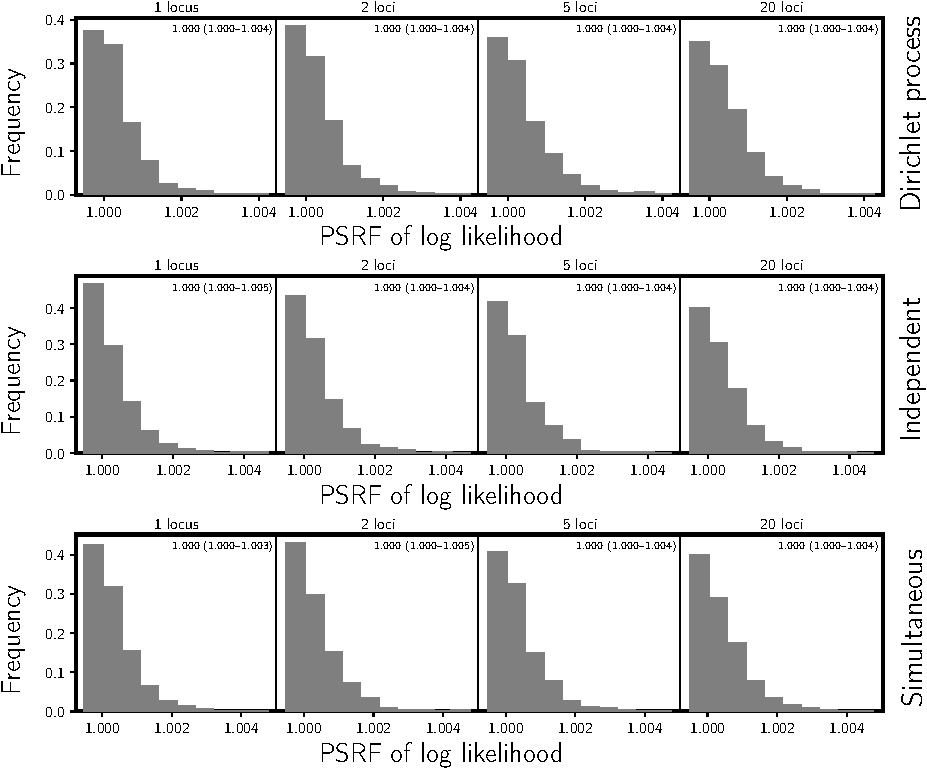
\includegraphics[width=\textwidth,height=0.9\textheight,keepaspectratio]{../images/from-project-repo/plots/tex-plot-grids/grid-psrf-lnl-histograms-cropped.pdf}
        \caption{
            The potential scale reduction factor \citep[PSRF; the square root
            of Equation 1.1 in][]{Brooks1998}
            for the log likelihood calculated from the last 1000
            samples of the four MCMC chains run for each simulation replicate.
            The mean PSRF across the 1000 simulation replicates is shown at the
            top right of each plot, followed by the range in parentheses.
        }
        \label{fig:psrflnl}
    \end{center}
\end{figure}

\begin{figure}[htbp]
    \begin{center}
        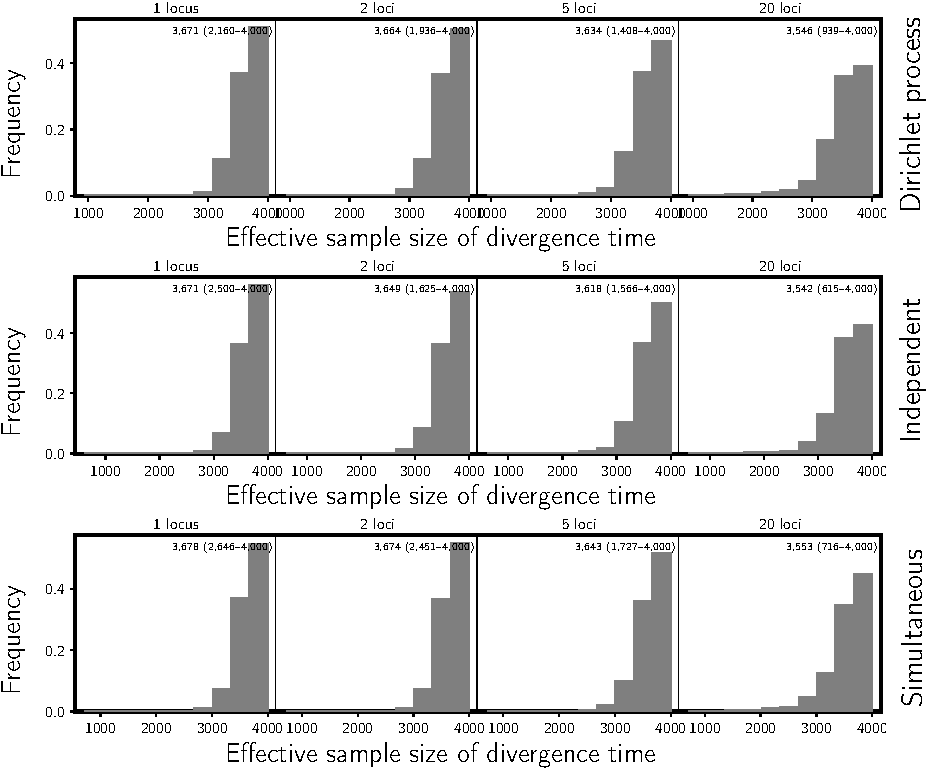
\includegraphics[width=\textwidth,height=0.9\textheight,keepaspectratio]{../images/from-project-repo/plots/tex-plot-grids/grid-ess-div-time-histograms-cropped.pdf}
        \caption{
            The effective sample size \citep[ESS;][]{Gong2014} for the
            divergence time parameter calculated from the last 1000 samples of
            the four MCMC chains run for each simulation replicate.
            The mean ESS across the 1000 simulation replicates is shown at the
            top right of each plot, followed by the range in parentheses.
        }
        \label{fig:essdivtime}
    \end{center}
\end{figure}

\begin{figure}[htbp]
    \begin{center}
        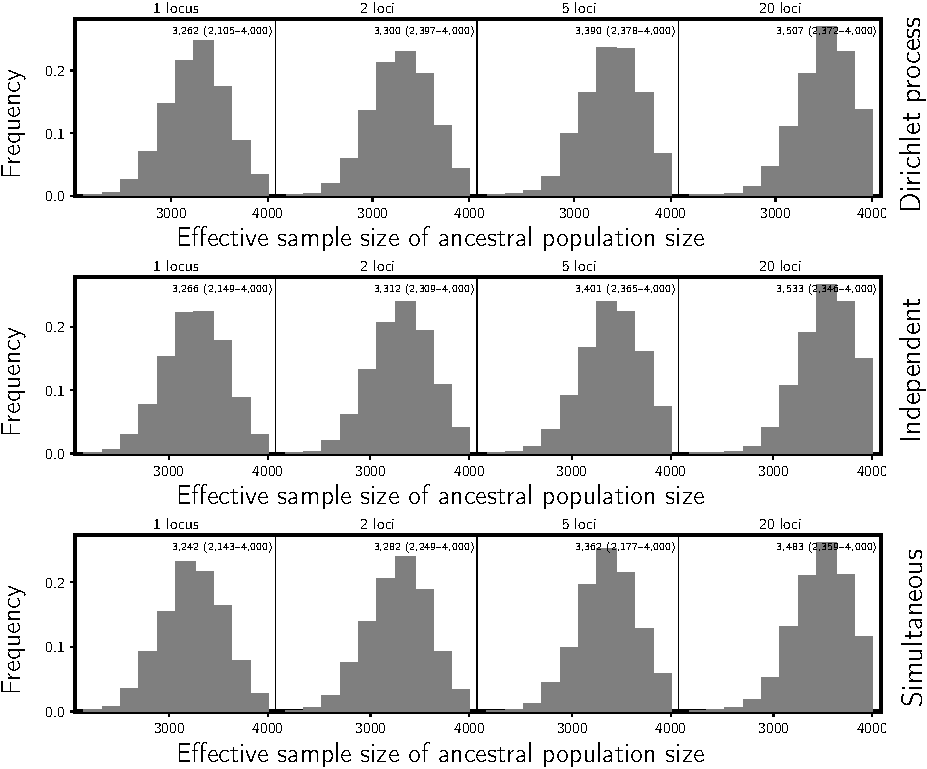
\includegraphics[width=\textwidth,height=0.9\textheight,keepaspectratio]{../images/from-project-repo/plots/tex-plot-grids/grid-ess-root-pop-size-histograms-cropped.pdf}
        \caption{
            The effective sample size \citep[ESS;][]{Gong2014} for the
            ancestral population size calculated from the last 1000 samples of
            the four MCMC chains run for each simulation replicate.
            The mean ESS across the 1000 simulation replicates is shown at the
            top right of each plot, followed by the range in parentheses.
        }
        \label{fig:essrootpopsize}
    \end{center}
\end{figure}

\begin{figure}[htbp]
    \begin{center}
        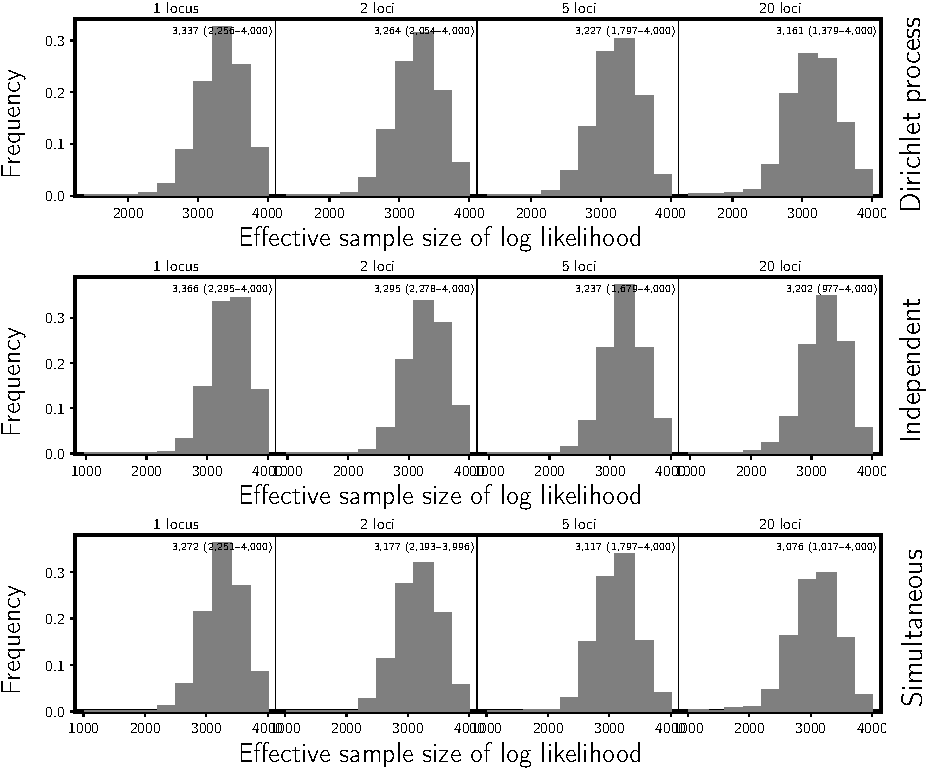
\includegraphics[width=\textwidth,height=0.9\textheight,keepaspectratio]{../images/from-project-repo/plots/tex-plot-grids/grid-ess-lnl-histograms-cropped.pdf}
        \caption{
            The effective sample size \citep[ESS;][]{Gong2014} for the
            log likelihood calculated from the last 1000 samples of
            the four MCMC chains run for each simulation replicate.
            The mean ESS across the 1000 simulation replicates is shown at the
            top right of each plot, followed by the range in parentheses.
        }
        \label{fig:esslnl}
    \end{center}
\end{figure}


%TC:endignore

\end{document}
